\section{Motivation}
\label{sec:motivation}

\begin{itemize}
	\item Motivate why we can't use QCD
	\item Highlight the impact of bkg syst in the current analysis
	\item Key modelling assumption: The properties of QCD are continuous across the $(m_{H1},m_{H2})$ plane
	\item Explain the starting point for these studies
\end{itemize}

\hl{TO DO: J explain how we're training before Xwt, and doing additional bkg validation studies}

The physical laws of the mulit-jet and $t\bar{t}$  background processes dominating our background are smoothly varying across the $(m_{H1}, m_{H2})$ massplane defining our SR.  We use this smooth variation from the underlying physics as a key inductive bias for training a generative model to constrain the \HH kinematics inside of the SR by training on the kinematics of events outside of the SR.

We show a set of results from the validation regions used for the recent $HH \rightarrow 4b$ analysis \cite{HDBS-2019-29}.
We are just looking at the modeling for the ggF channel, and since a smooth massplane is a key starting point for these studies, all trainings are done \emph{before} the \Xwt cut.


\begin{figure}[ht]
    \centering
    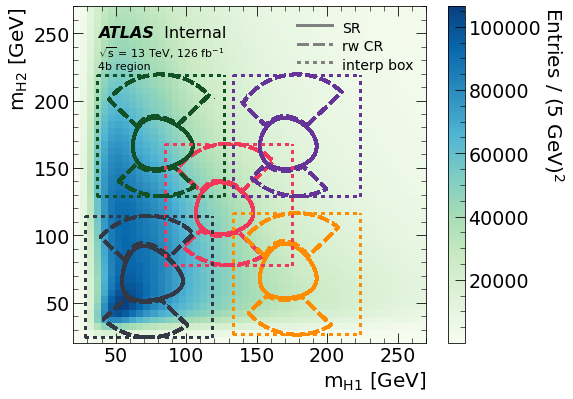
\includegraphics[width=0.5\textwidth]{figures/flows/fullmassplane_shift_regs_all}  
    %\subfloat{ 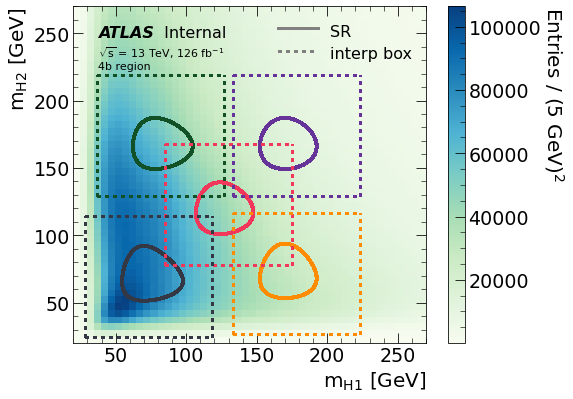
\includegraphics[width=0.44\textwidth]{figures/flows/fullmassplane_shift_regs_rw_all} }   <- this plot doesn't show the rw lines
    \caption{ Illustration of the interpolation regimes. The pink (solid) circle shows the nominal 4b SR, with the pink dotted line showing the interpolation bounding box. The quadrants used to define the reweighing are also shown in the pink dashed crescents. The shifted regions used as validation tests of the method are shown in the blue, orange, green and purple overlays. }
    \label{fig:fullmassplane-shift-regs}
\end{figure}


% Not including b/c rev deta won't be my default here
%\begin{figure}[hbt]
%    \centering
%    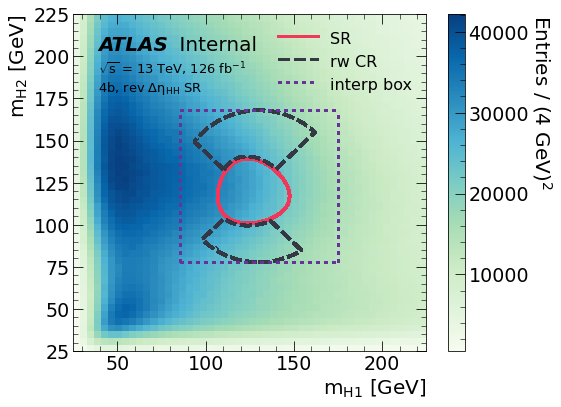
\includegraphics[width=0.9\textwidth]{figures/flows/rev_deta/fullmassplane_all.png}%{figures/intro/V1/massplane_dat_all_4b_ggf_preXwt.png}
%    \caption{Massplane with the 4b reversed $\Delta \eta_{HH}$  analysis selection. The pink circle shows our blinded SR that we want to interpret the \HH kinematics in. The dotted purple line shows the region where the GP+flows fit is derived in, while the dashed navy line shows where the region where the reweighting is derived.}
%        \label{fig:ggF-massplanes-allYrs-dat-4b-preXwt}
%\end{figure}




